% This is samplepaper.tex, a sample chapter demonstrating the
% LLNCS macro package for Springer Computer Science proceedings;
% Version 2.20 of 2017/10/04
%
\documentclass[runningheads]{llncs}
%
\usepackage{graphicx}
\usepackage{placeins}
% Used for displaying a sample figure. If possible, figure files should
% be included in EPS format.
%
% If you use the hyperref package, please uncomment the following line
% to display URLs in blue roman font according to Springer's eBook style:
% \renewcommand\UrlFont{\color{blue}\rmfamily}

\begin{document}
%
\title{Immortals 2020 Extended Team Description Paper}
%
%\titlerunning{Abbreviated paper title}
% If the paper title is too long for the running head, you can set
% an abbreviated paper title here
%
\author{Omid Najafi\inst{1} \and
MohammadAli Ghasemieh\inst{2} \and
Mehran Khanloghi\inst{3} \and
AmirMahdi Matin\inst{3} \and
AliReza Mohammadi\inst{3} \and
AmirMahdi Torabian\inst{4}}
%
\authorrunning{Immortals Robotics}
% First names are abbreviated in the running head.
% If there are more than two authors, 'et al.' is used.
%
\institute{Sharif University of Technology \and
Pars University of Art \and
University of Tehran \and
University of Science and Technology \\
\url{http://www.immortals-robotics.com}
}
%
\maketitle              % typeset the header of the contribution
%
\begin{abstract}
%The abstract should briefly summarize the contents of the paper in
%15--250 words.
This paper describes the recent work done by the Immortals Robotics Team for the upcomming competitions including the RoboCup 2020.

\keywords{RoboCup 2020  \and Small Size League}
\end{abstract}
%
%
%
\section{Introduction}
The Immortals Robotics Team consists of art and engineering students from different Persian universities.
The team was established in 2007 with the focus of designing a robust robot while meeting all the requirements according to the Small Size League rules. The teams strategy is to adopt itself with all the rule changes in order to experience the new challenges. This makes the team to take part in the division-A which is intended for the advanced teams of the league~\cite{ref_website}.

In the previous years the team reached close enough to a SSL robot design and solved most of the issues found in the previuos designs. The process of upgrading the robot can be seen in the previous years TDPs and ETDPs~\cite{ref_ETDP2019} of this team. The readers who are interested in designing or upgrading a SSL robot are encouraged to study the previous papers of this team.

\begin{figure}
\centering
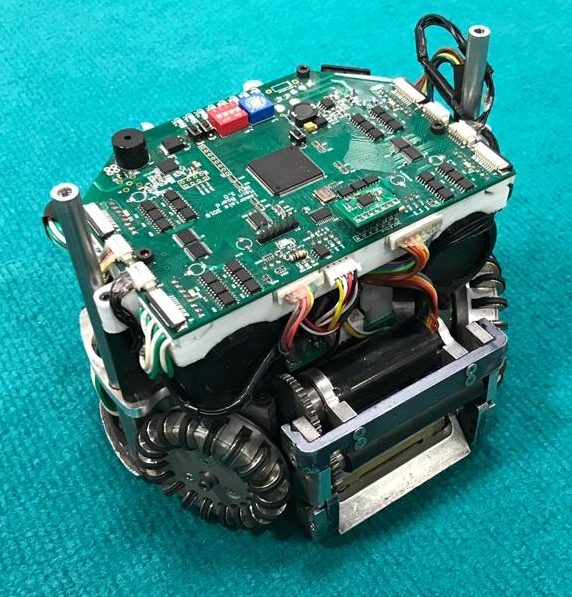
\includegraphics[width=10cm]{images/std_robot.jpeg}
\caption{Immortals current robot.} \label{fig_std_robot}
\end{figure}

This year the team had the chance to improve the AI software design which is the core program runing on a desktop or laptop copmuter and is the means to navigate each robot. The robots move and take actions defined by this program. Other enhancements, however, have been continued to be made to the robots mechanics and electonics which will be explained further.

\section{Software}
This year the main software also known as the AI software is redesigned in order to be more understandable and extandable. In previous years the software core was the same for each year but with slight changes according to rules or new referee commands. The new members who wanted to implement a new idea in the software needed to spend a great amount of time to uderstand the methods to use for the robot navigation and data input.

The inputs for the software are vision data, referee commands and a configuration file which tells the initial parameter values for the network and match conditions. The outputs are simple navigation commands to the robots such ass move in a direction with this magnitude of speed or kick the ball with this amount of force.

The new software is written in C++ same as the previous one. The only reason to use this language is the performance and easy to extend capabilities of i. For example the ability to optimize the code by using GPUs are well defined in this language.

\subsection{Finite-State Machine} 
After a few years of experience in the Small Size League as a software designer the key idea that every team is looking to implement is to make the robots to take the correct action at the exact time and condition. If the actions are perfomed correctly, the robots will accomplish their task which is scoring a goal or preventing the opponent from scoring. Unfortunately, there are many conditions that can happen in a match and each one has its own set of solutions these solutions are the sequence of commands which are given to a set of robots. For the software designer it may be hard to implement the solutions with a group of \textit{IF} conditions and no special structures.

In order to simplify the implementation for multiple software designers in the team, a Finite-State Machine implementation structure has been introduced. This gives a great flexibility and readablity of implementation in the code. Each state is implemented by a single person and each state is connected to other states by a condition or conditions. This makes the implementation more easily to probe if solution does not work as expected the transmitions in the states can be viewed in the logs and the creator of the state can be found.

Each state is basically a function which will be called whenever a complete picture of a field is received from the vision. The input of the function, or state, are the vision data.  
In each state, the set of commands which have to be given to the robots in the field are defined and if there is a condition which a state transmition is requiered the next state will be defined to be called next time.
Table~\ref{tab1} shows a sample group of commands which can be used in every state:

\begin{table}
\caption{Example commands which can be used in every state.}\label{tab1}
\begin{tabular}{|p{7.5cm}|p{6cm}|}
\hline
Function &  Explanation \\
\hline
{\itshape Navigate2Point(robot, destination, maxSpeed)} & Navigate the robot to a destination.\\
{\itshape ERRTNavigate2Point(robot, destination, maxSpeed)} & Navigate the robot while avoinding obstacles.\\
{\itshape Mark(robot, oppRobot)} & Position between the goal and an opponent robot.\\
{\itshape FetchBall(robot, point)} & Navigate the robot to a position on line which the ball is moving on and most close to the \itshape{point} argument.\\
{\itshape CircleBall(robot, radius, angle)} & Position robot on a circle around the ball in a specific angle.\\
{\itshape face(robot, point)} & Face the robot towards a point.\\
{\itshape Chip(robot, power)} & Robot should perform a chip kick whenever the ball was intercepted.\\
{\itshape Direct(robot, power)} & Robot should perform a direct kick whenever the ball was intercepted.\\
%Title (centered) &  {\Large\bfseries Lecture Notes}\\
%1st-level heading &  {\large\bfseries 1 Introduction}\\
%2nd-level heading & {\bfseries 2.1 Printing Area}\\
%3rd-level heading & {\bfseries Run-in Heading in Bold.} Text follows\\
%4th-level heading & {\itshape Lowest Level Heading.} Text follows\\
\hline
\end{tabular}
\end{table}

As shown in Table~\ref{tab1} the commands are fairly simple to be understood. This simple implementation saves a great amount of time for the programmers to extend or debug the code.

\subsection{Debugging Tools}
Another experience with the previous AI software was the process of debugging the algorithems and, in general, the code itself. To overcome this problem, a logging protocol has been implemented which defines the messages that are sent from the AI software while operating. Using that protocol, whenever a computer is running the AI software and is connected to the network any other computer in the same network can run a logging software and monitor the AI software's parameters including not just the simple inputs from the vision, but also the state, predictions of the algorithems and et al.

Fig~\ref{fig1_plotter} Shows a simple plotter which uses this protocol to visualize the changes in the speed and commanded velocity of a single robot. The plotter is a simple python script while the AI is written in C++ as mentioned before.

\begin{figure}
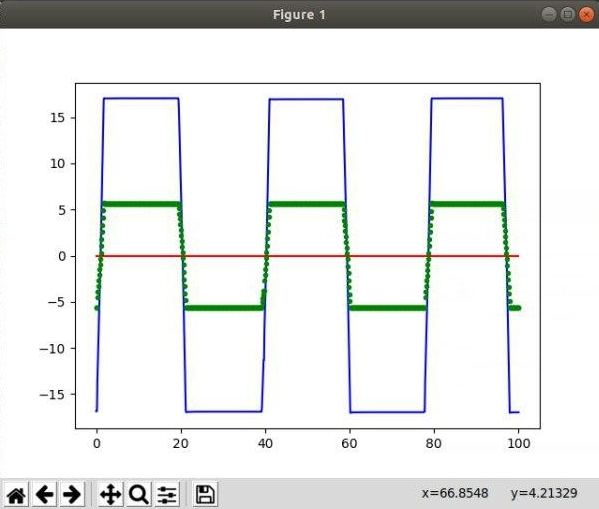
\includegraphics[width=\textwidth]{images/plotter.jpg}
\caption{An example logging program compatible with the new AI software.} \label{fig1_plotter}
\end{figure}

\section{3D printed robot}
As mentioned in the previous years team description paper[], A new type of robot was introduced to the league by this team in order to reduce the time of manufacturing the robots. This idea benefits teams in terms of energy and time of manufacturing.

The design of the 3d printed robots where published and are available for teams and individuals to use~\cite{ref_opensource}. The designs are being updated to increase robustness. Though, the robustness of a 3d printed robot is incomparable with a usual SSL robot which is assembled with metal parts.

\section{Kickers Solenoid}
Before 2018 the limitations of the ball velocity was 8m/s which limited the robots to not shoot more than this velocity. In order for robots to kick a ball this much fast a strong shooting system including capacitors and solenoids where required to be used. Since RoboCup 2018, Montréal, Canada, the maximum speed limit has been decreased to 6.5m/s which makes teams to wonder if they want to redesign their robots kicking system in order to optimize the space consumption or battery power in their robot. This year the Immortals robots kicking system has been modified in order to optimize the energy consumption from the battery. This way robots have the chance to stay longer in a match without the need of their battery to be changed.

\begin{figure}
\centering
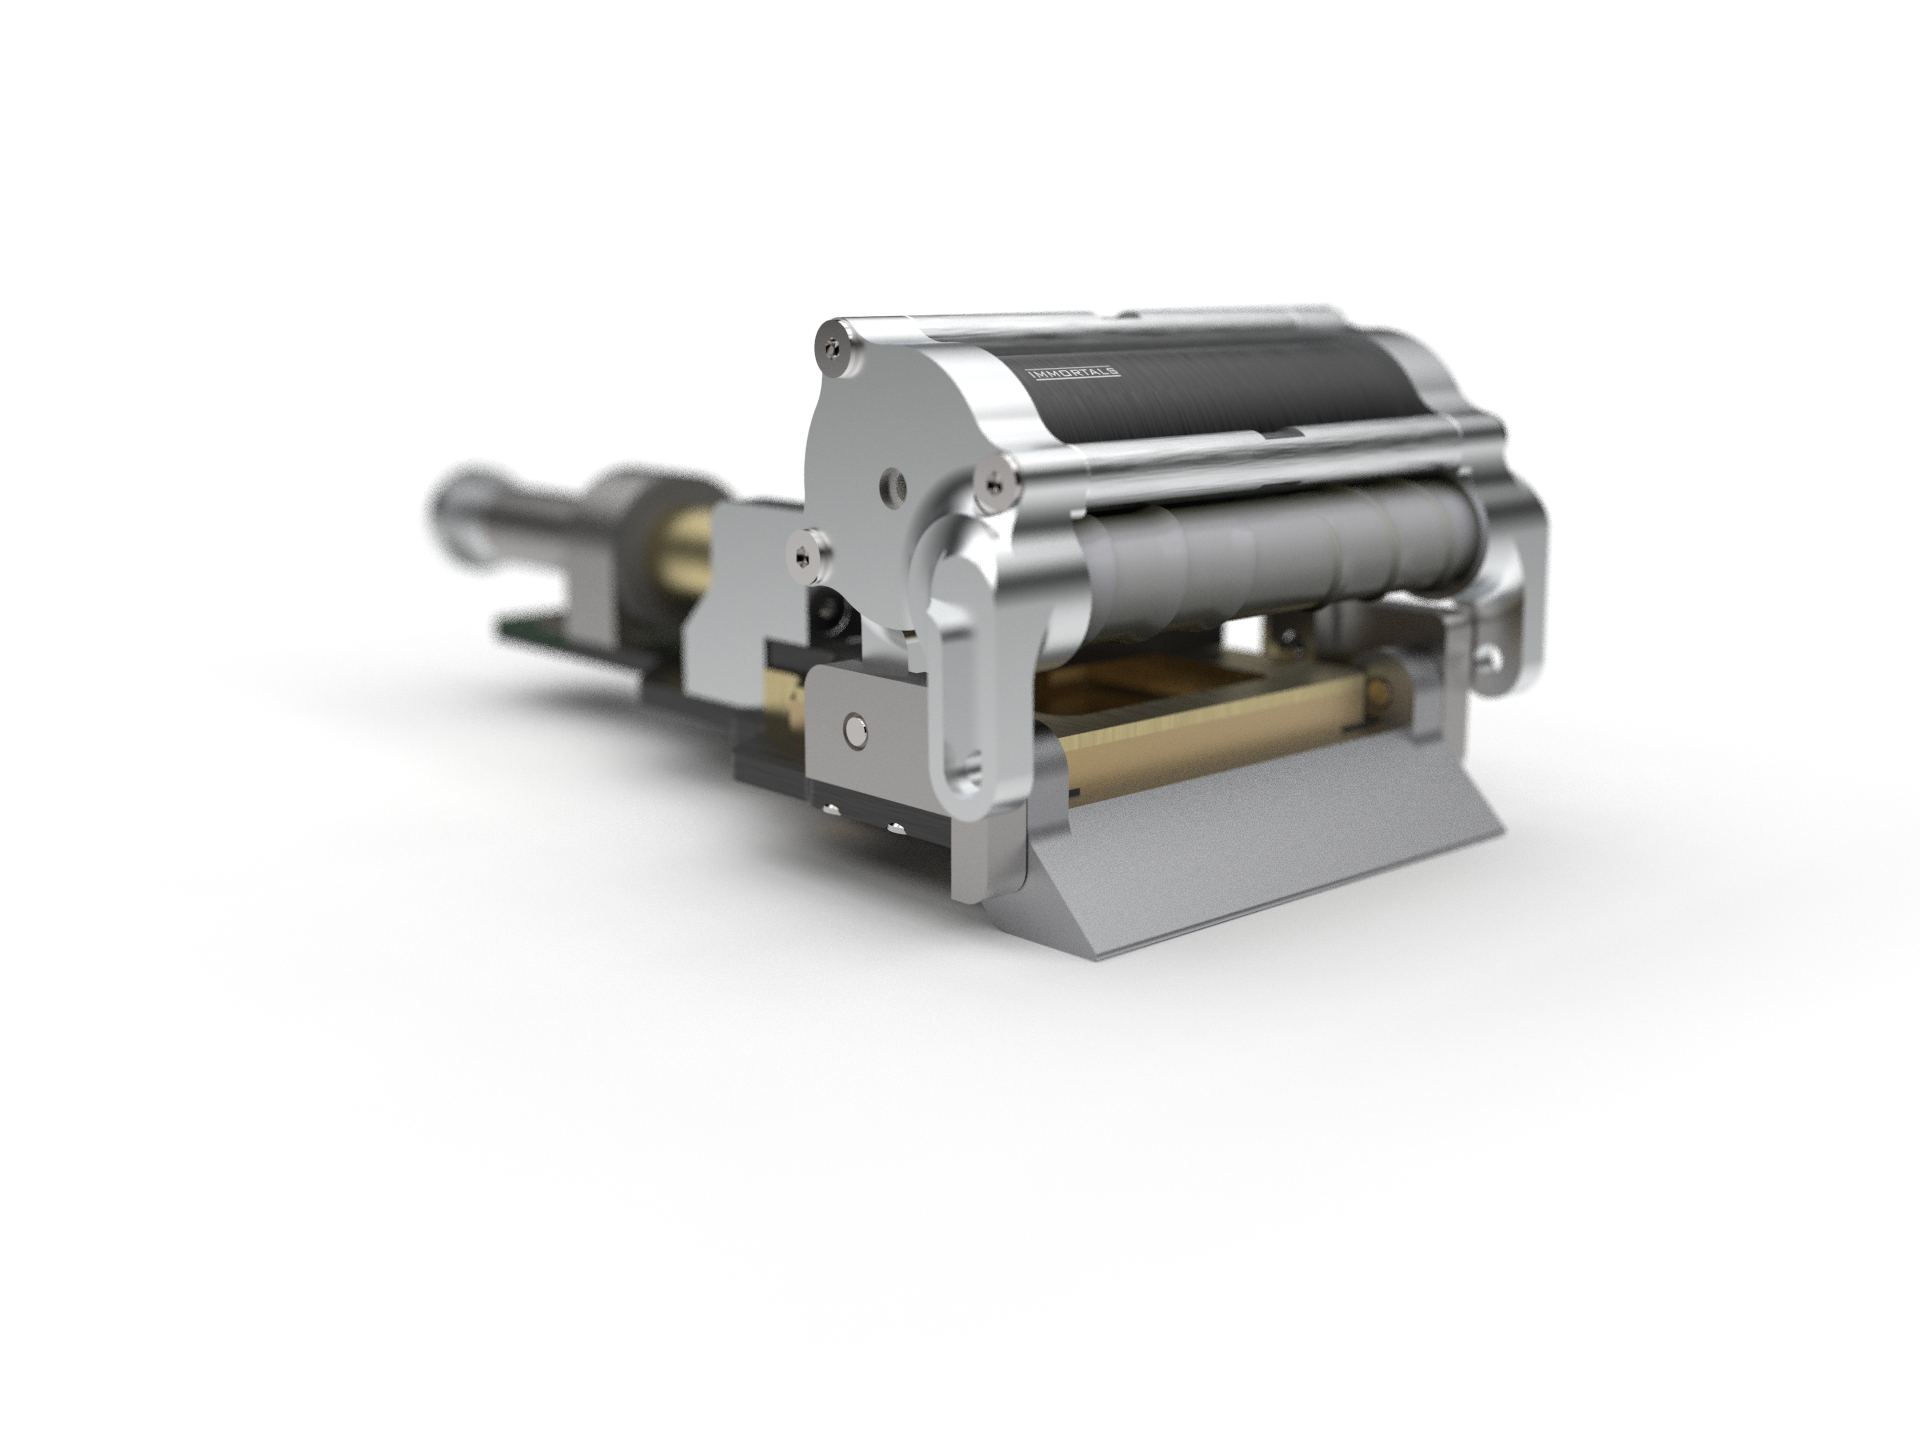
\includegraphics[width=10cm]{images/kicking_system.jpg}
\caption{The latest kicking system of the Immortals robots.} \label{fig_Kick_Sys}
\end{figure}

To understand the upgrade process of the shooting system, the reader is referred to the previous years (E)TDPs of this team.

This year it has been decided to redesign the shooting solenoid which is the part that converts the electrical power to a magnetic field and thus it will move the metal plunger towards the ball to be kicked. The previous solenoid had a low resistance in order to pass a higher current through it which will result in a higher and less controllable speed. This part has been modified in a way that less current is flown in the solenoid to save more enegry and generate less heat. Although the kicking power will decrease, it will not disable the robot to kick the ball to less than 6.5m/s. Both old and new versions of the solenoids are shown in Fig~\ref{fig_solenoid}.

\begin{figure}
\centering
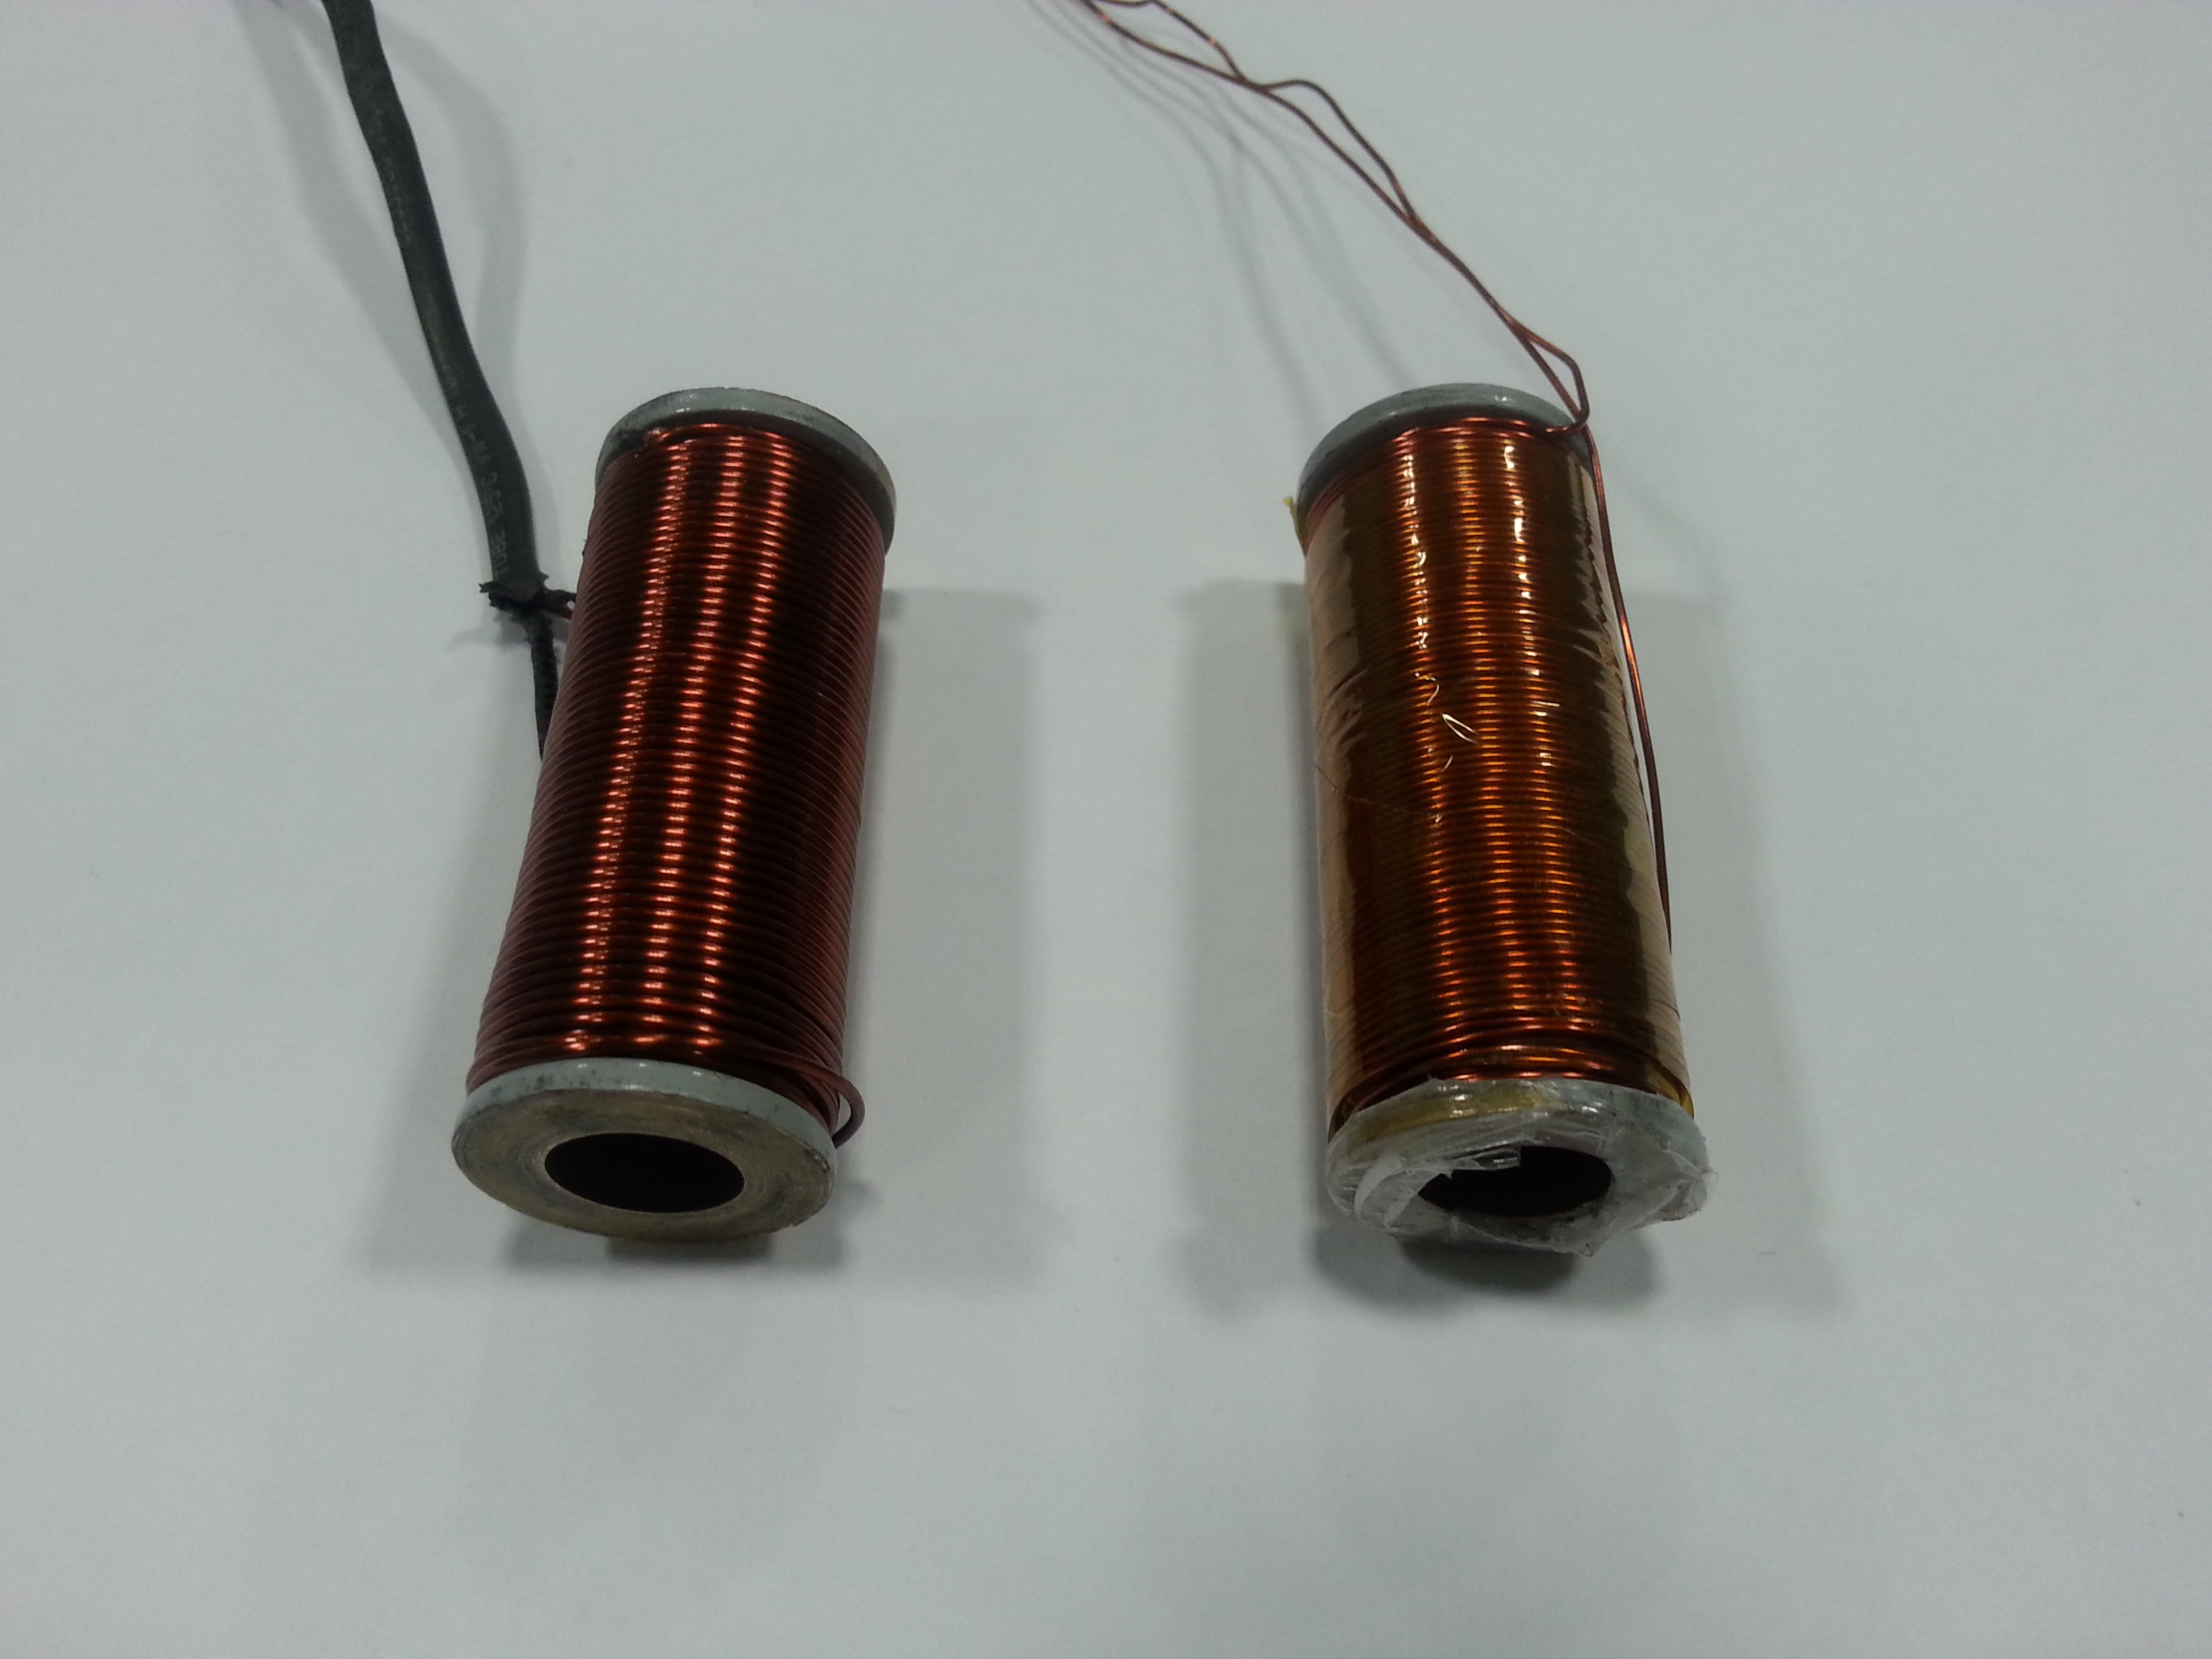
\includegraphics[width=10cm]{images/solenoid.jpg}
\caption{The old solenoid(Left) and the new solenoid(Right).} \label{fig_solenoid}
\end{figure}


\begin{figure}
\centering
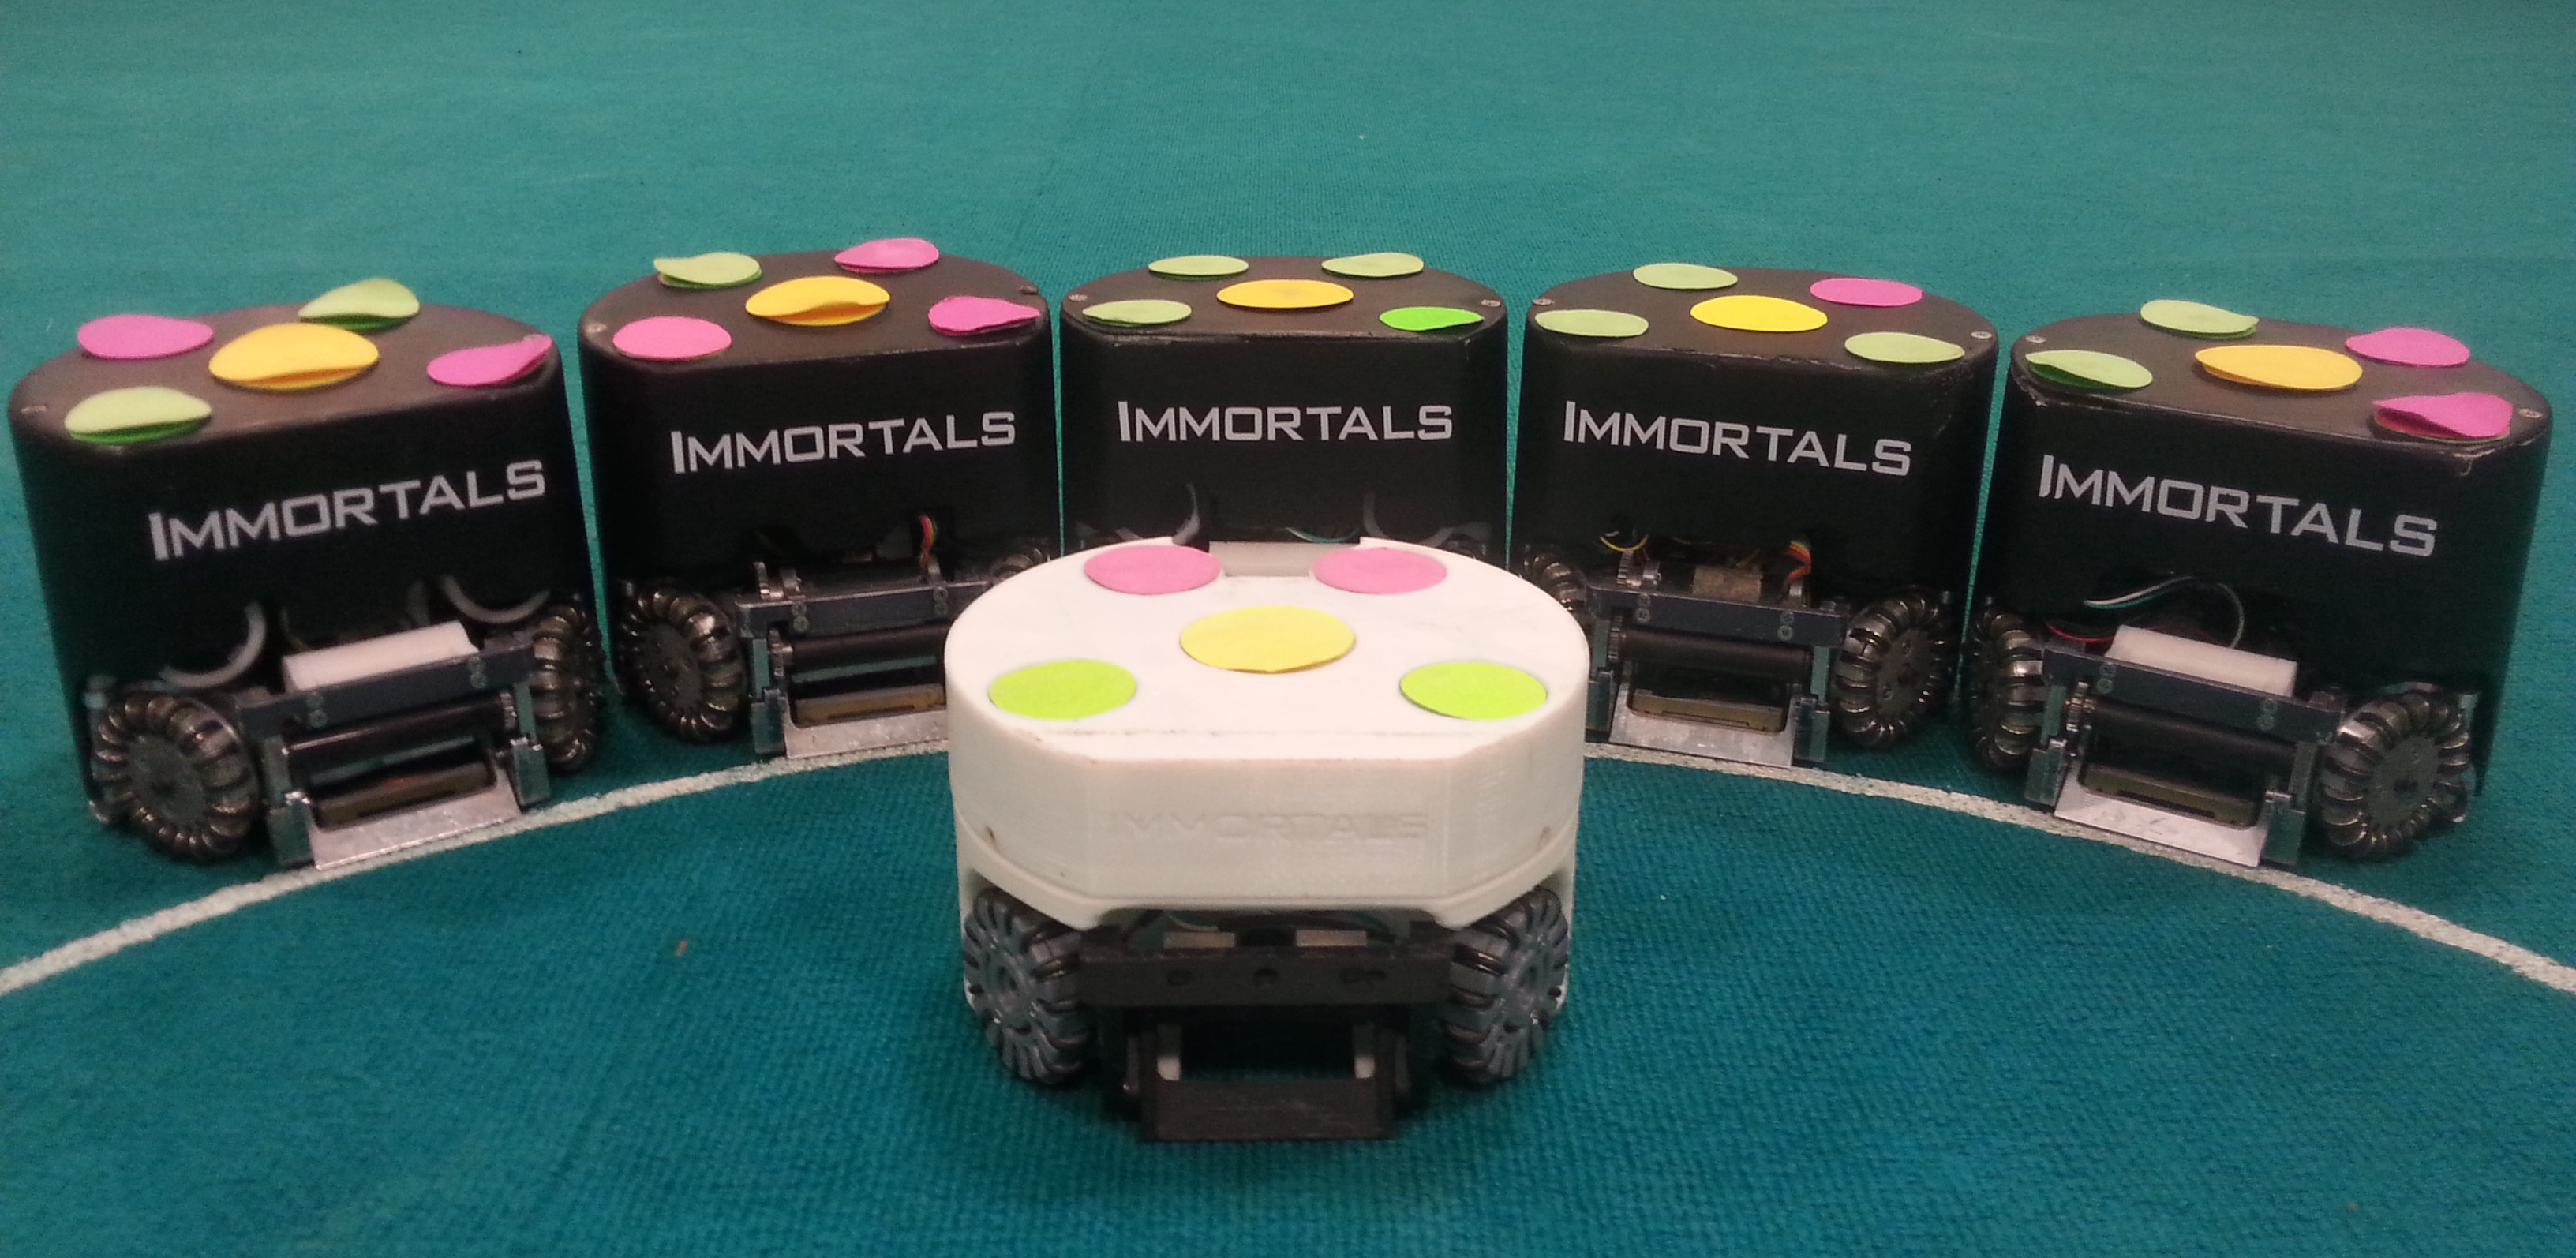
\includegraphics[width=10cm]{images/5plus1.jpg}
\caption{Five old robots and a single 3D printed robot at the front.} \label{fig_5plus1}
\end{figure}



\newpage
\begin{thebibliography}{8}
\bibitem{ref_website}
Immortals Robotics WebSite, \url{http://www.immortals-robotics.com}.

\bibitem{ref_ETDP2019}
Najafi, O.,Ghasemieh, M.A. and others:Immortals 2019 Team Description Paper

\bibitem{ref_opensource}
Immortals Open Source Project. \url{https://github.com/Ma-Ghasemieh/Immortals\_ssl\_opensource\_mech}.

\bibitem{ref_opensource}
Immortals Open Source Publish in RoboCup 2016. \url{https://github.com/lordhippo/immortalsSSL}.

\end{thebibliography}
\end{document}
